\documentclass[fleqn,10pt]{SelfArx} % Document font size and equations flushed left

\usepackage{float}
\usepackage{graphicx}
\usepackage{caption}
\graphicspath{{../figures/}}


\def\numTools{498}
%cat meanRankSpeedData.tsv | cut -f 4 | grep -v ^method$ | wc -l
\def\numBenchmarkPubs{68}
%cat speed-vs-accuracy-toolRanks2005-2020.tsv | cut -f 1 | sort  | uniq | grep -E '[0-9]'  | wc -l
\def\numBenchmarks{133}
%cat rawRankSpeedData2005-2020.tsv | cut -f 1 | grep -v ^testId$ | uniq -c | wc -l


\newcommand{\beginsupplement}{%
        \setcounter{table}{0}
        \renewcommand{\thetable}{S\arabic{table}}%
        \setcounter{figure}{0}
        \renewcommand{\thefigure}{S\arabic{figure}}%
     }

\definecolor{color1}{RGB}{0,0,90} % Color of the article title and sections
\definecolor{color2}{RGB}{0,20,20} % Color of the boxes behind the abstract and headings

\JournalInfo{Supplementary Text} % Journal information ``Journal, Vol. XXI, No. 1, 1-5, 2015''
\Archive{ } % Additional notes (e.g. copyright, DOI, review/research article)


\PaperTitle{Supplementary results for: Sustained software development, not number of citations or journal choice, is indicative of accurate bioinformatic software} % Article title

\Authors{Paul P. Gardner\textsuperscript{1,2}*, James M. Paterson\textsuperscript{3}, Stephanie McGimpsey\textsuperscript{4}, Fatemeh Ashari-Ghomi\textsuperscript{5}, Sinan U. Umu\textsuperscript{6}, Aleksandra Pawlik\textsuperscript{7},
Alex Gavryushkin\textsuperscript{8}, Michael A Black\textsuperscript{1}
} % Authors

\affiliation{\textsuperscript{1}\textit{Department of Biochemistry, University of Otago, Dunedin, New Zealand.}} % Author affiliation
\affiliation{\textsuperscript{2}\textit{Biomolecular Interaction Centre, University of Canterbury, Christchurch, New Zealand.}}
\affiliation{\textsuperscript{3}\textit{Department of Civil and Natural Resources Engineering, University of Canterbury, Christchurch, New Zealand.}}
\affiliation{\textsuperscript{4}\textit{Parasites and Microbes, Wellcome Sanger Institute, Wellcome Genome Campus, Hinxton,
8 Cambridgeshire, CB10 1RQ, UK.}}
\affiliation{\textsuperscript{5}\textit{Research Group for Genomic Epidemiology, National Food Institute, Technical University of Denmark, Kongens Lyngby, Denmark.}}
\affiliation{\textsuperscript{6}\textit{Department of Research, Cancer Registry of Norway, Oslo, Norway.}} % Author affiliation
\affiliation{\textsuperscript{7}\textit{New Zealand eScience Infrastructure, 49 Symonds St, Auckland, New Zealand.}}
\affiliation{\textsuperscript{8}\textit{Department of Computer Science, University of Otago, Dunedin, New Zealand.}} % Author affiliation

\affiliation{*\textbf{Corresponding author}: paul.gardner@otago.ac.nz} % Corresponding author

\Keywords{computational biology --- accuracy --- benchmarks --- meta-analysis --- software development} % Keywords - if you don't want any simply remove all the text between the curly brackets
\newcommand{\keywordname}{Keywords} % Defines the keywords heading name

%----------------------------------------------------------------------------------------
%	ABSTRACT
%----------------------------------------------------------------------------------------

\Abstract{In the below we provide additional results for our
  investigation of computational biology benchmarks.}

\begin{document}

\flushbottom % Makes all text pages the same height
\maketitle % Print the title and abstract box
%\tableofcontents % Print the contents section

\thispagestyle{empty} % Removes page numbering from the first page

%----------------------------------------------------------------------------------------
%	ARTICLE CONTENTS
%----------------------------------------------------------------------------------------

\onecolumn
\beginsupplement

\section*{Literature mining} % The \section*{} command stops section numbering


\begin{figure}[H]
\centering
\includegraphics[height=0.7\textheight]{litMiningFlowDiagram-edited.pdf}
\caption{In order to improve the identification of benchmark articles
  that rank both accuracy and speed we developed a tool for ranking
  PubMed articles based upon word association scores (measured in
  ‘bits’). In brief, keywords were extracted from titles and abstracts
  for both training (in this case benchmark articles) and background
  articles (articles published between 2013 and 2015 with
  “bioinformatics” in the title or abstract). Log-odds ratios were
  computed for each keyword (measured in ‘bits’). Candidate articles
  that matched a hand-selected list of keywords associated with
  benchmarks: \texttt{((bioinformatics OR (computational AND biology)) AND (algorithmic OR algorithms OR biotechnologies OR computational OR kernel OR methods OR procedure OR programs OR software OR technologies)) AND (accuracy OR analysis OR assessment OR benchmark OR benchmarking OR biases OR comparing OR comparison OR comparisons OR comparative OR comprehensive OR effectiveness OR estimation OR evaluation OR metrics OR efficiency OR performance OR perspective OR quality OR rated OR robust OR strengths OR suitable OR suitability OR superior OR survey OR weaknesses OR correctness OR correct OR evaluate OR competing OR competition) AND (complexity OR cputime OR runtime OR walltime OR duration OR elapsed OR fast OR faster OR perform OR performance OR slow OR slower OR speed OR time OR (computational AND resources))}. These 
  were then scored and ranked with a “sum of bits”
  score. High ranking articles were then inspected, those that met our
  criteria were added to the training set, those that did not were
  added to the background set of articles.}
\label{fig:flow}
\end{figure}



\begin{figure}[H] \centering
\includegraphics[width=0.99\textwidth]{wordScores.pdf} \caption{The 40
  highest ({\bf right}) and lowest ({\bf left}) scoring words that are associated with
  bioinformatic benchmark articles from the training benchmark articles,
  compared to the background articles. The log-odds ratios (measured
  in bits) are indicated on the y-axis. }
\label{fig:wordScores} \end{figure}


%% \clearpage
%% \newpage

%% \section*{R code ...}

%% {\tiny
%% \begin{verbatim}

%% \end{verbatim}
%% }


\clearpage
\newpage

\section*{Data visualisations} % The \section*{} command stops section numbering

\begin{figure}[htb!]
\centering
\includegraphics[width=0.95\textwidth]{supplementary-figures-small.pdf}
\caption{The distributions for the measures that have been proposed to be
predictive of software quality used in this study. These
are, reading from left to right, top to bottom:
Accuracy -- the mean normalised accuracy rank for each benchmarked method;
Speed -- the mean normalised speed rank for each benchmarked method;
JH5 -- the Journal H5 index to the highest impact journal that has published a manuscript describing a method, data from GoogleScholar 2020 Metrics;
Cites -- the number of citations to the most cited manuscript describing a method, data from GoogleScholar;
H-index -- the H-index for the highest profile corresponding author from the manuscripts describing a method, data from GoogleScholar User Profiles;
M-index -- the M-index (H-index/(\#years since first publication)) for the highest profile corresponding author from the manuscripts describing a method, data from GoogleScholar User Profiles;
Relative ages -- for different tools, for each benchmark tools were ranked based upon publication dates, these ranks were normalised to lie between 0 and 1.
Relative \#citations -- within each benchmark, what is the relative age of each tool, this corrects for older research fields (e.g. sequence alignment) vs newer research fields (e.g. single-cell sequencing);
Year published -- the first year each software tool was published;
Version -- the most resent version number for each tool;
Commits -- the number of commits to Github;
Contributors -- the number of contributors to a Github repository;
\#Issues -- the number of open and closed issues for each Github repository;
\%Open issues -- the pecentage of issues that remain open for each Github repository;
\#Pull requests -- the number of pull requests to a Github repository;
\#Forks -- the number of times a Github repository has been forked;
}
\label{fig:metricDistributions}
\end{figure}


\begin{figure}[htb!]
\centering
\includegraphics[width=0.95\textwidth]{supplementary-distributions-permuted.pdf}\\
\caption{The distributions for the permuted accuracy ({\bf left}) and speed ({\bf right}) values, where accuracy and speed ranks have been normalised to lie between 0 and 1. 
}
\label{fig:metricDistributionsPerm}
\end{figure}

\clearpage

\begin{figure}[H]
\centering
\includegraphics[width=0.95\textwidth]{supplementary-figures-pairs.pdf}
\caption{Dot plots for each feature relative to every other feature
  (accuracy, speed, JH5, citations, H-index, M-index, relAge,
  relCites, yearPublished, version, commits, contributors, \#Issues,
\%Open issues, \#Pull requests, and the \#Forks).
}
\label{fig:metricPairs}
\end{figure}


\begin{figure}[H]
\centering
\includegraphics[width=0.45\textwidth]{spearmanBarplot.pdf}
\includegraphics[width=0.45\textwidth]{spearmanBarplotSpeed.pdf}
\caption{The correlation between method accuracy ({\bf left}) and
  method speed ({\bf right}) and measures we expected to be
  predictive of software quality. E.g. author reputation measures
  (H-index, M-index), journal reputation (JH5 and JIF), number of
  users (citations and relative citations) or the recency of methods
  (year and relative age).  The correlations were estimated using
  Spearman's $\rho$. The signficant relationships are indicated with a
  ``*''. }
\label{fig:S2}
\end{figure}


%% \begin{figure}[H]
%% \centering
%% 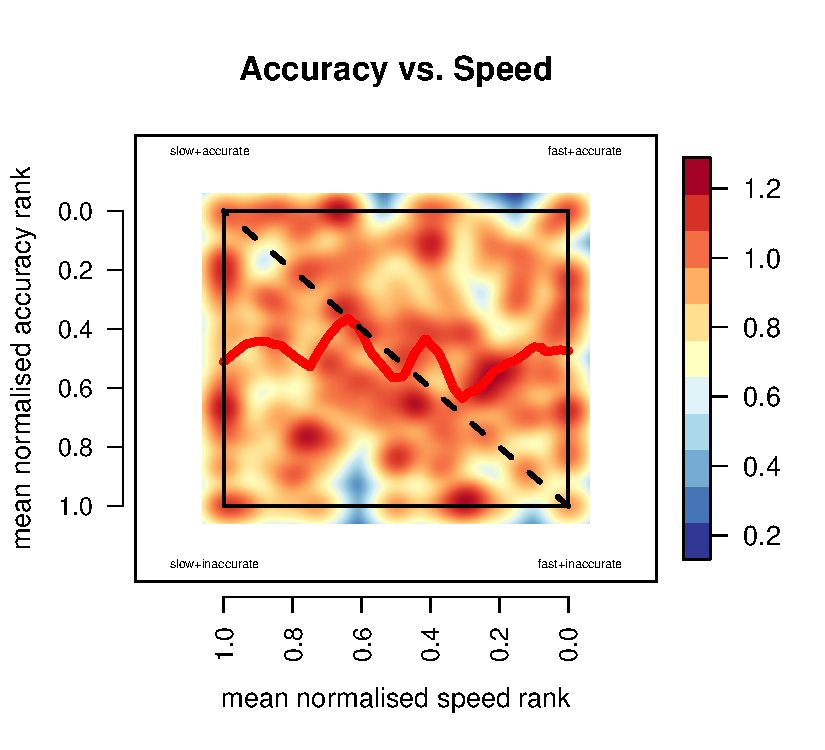
\includegraphics[width=0.5\textwidth]{smoothScatter-speed-vs-accuracy.pdf}
%% \caption{A smoothed color density representation of a scatterplot of
%%   normalised speed ranks and normalised accuracy ranks. Dark red
%%   regions are indicative of of a high density of points, blue shades
%%   indicate the reverse. The expected inverse relationship between
%%   speed and accuracy is indicated with a dashed black line, points
%%   above this line could be considered comparatively fast and accurate,
%%   points below are the reverse. A locally weighted regression (lowess)
%%   curve is shown in red.}
%% \label{fig:smoothScatterAccSpeed}
%% \end{figure}

%% \begin{figure}[H]
%% \centering
%% 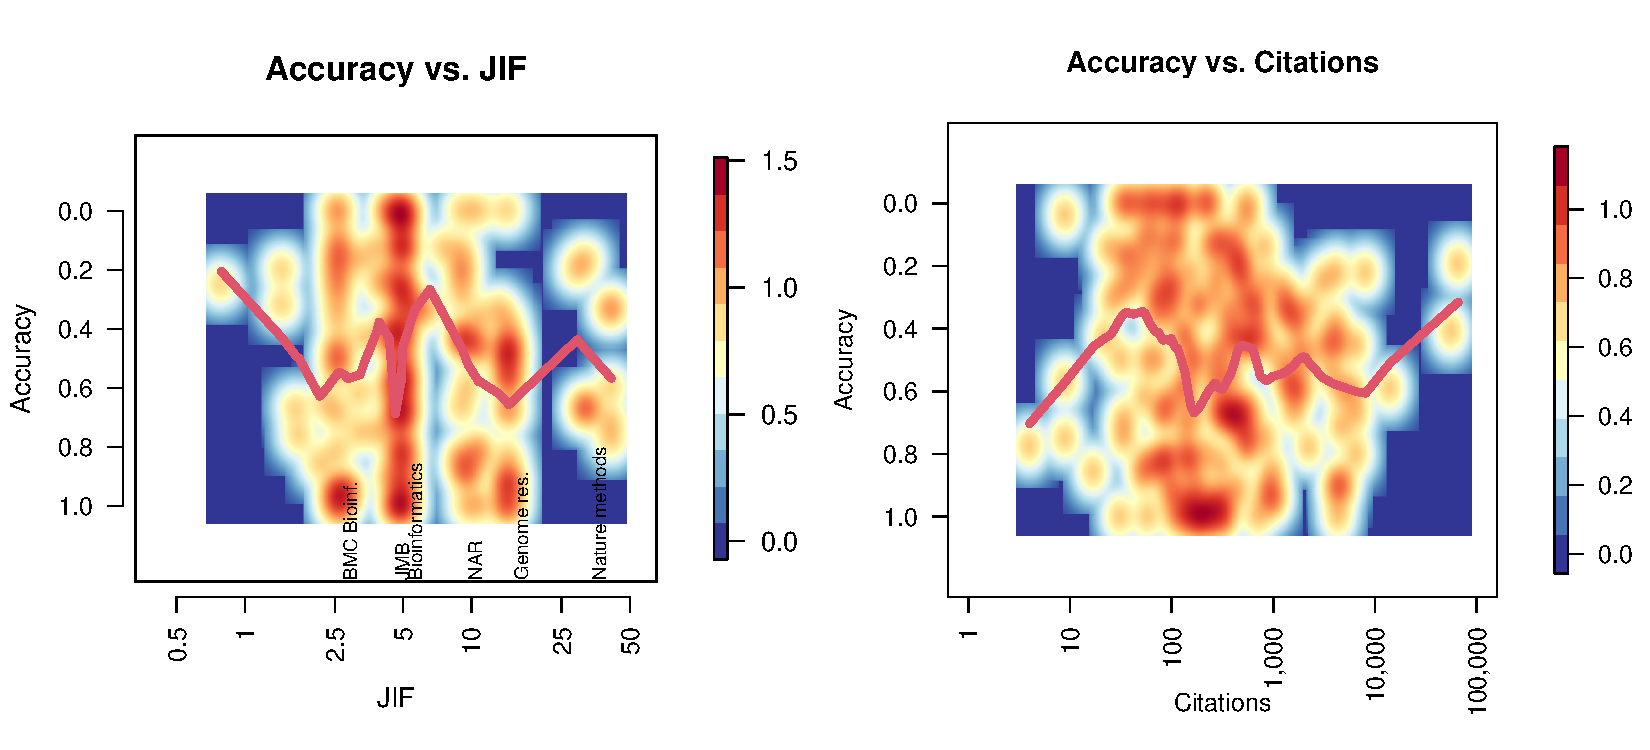
\includegraphics[width=0.85\textwidth]{smoothScatters.pdf}
%% \caption{A smoothed color density representation of a scatterplot of
%%   journal impact factors (JIF) on the left and number of citations on
%%   the right vs normalised accuracy ranks. As above, dark red regions
%%   are indicative of of a high density of points, blue shades indicate
%%   the reverse. The JIF for journals that are major publishers of
%%   bioinformatic software are indicated on the left. }
%% \label{fig:smoothScatters}
%% \end{figure}



%% \begin{figure}[H]
%% \centering
%% \includegraphics[width=0.45\textwidth]{hindex-SpeedVsAccuracy-heatmap.pdf}
%% \includegraphics[width=0.45\textwidth]{cites-SpeedVsAccuracy-heatmap.pdf}
%% \caption{{\bf Citation metrics and software tool speeds/accuracies.} Heatmaps of normalised speed ranks and normalised accuracy
%%   ranks, both $x$ and $y$ dimensions are discretised into a $3 \times
%%   3$ matrix. The shading indicates different median citation-based
%%   feature scores (redder shade indicates a higher value).  The shading
%%   indicate median H-indices ({\bf left}) and $log_{10}(citations)$
%%   ({\bf right}). }
%% \label{fig:heatmaps}
%% \end{figure}


\begin{figure}[H]
\centering
%\includegraphics[width=0.45\textwidth]{relAge-speedAcc-jitterPlot.pdf}
%\includegraphics[width=0.45\textwidth]{relAge-SpeedVsAccuracy-heatmap.pdf}
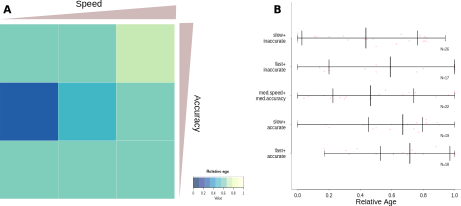
\includegraphics[width=0.95\textwidth]{relAge.pdf}
\caption{{\bf Relative software tool ages and speeds/accuracies.}
{\bf A.} A heatmap indicating the relative age
  of software in a range of relative accuracy and speed rankings. Blue
  colours indicate an abundance of older software tools in an accuracy
  and speed category, while light colours indicate younger software in
  an accuracy and speed category.
  {\bf B.} Jitter-plots for the relative age distribution
  for software tools in each of the 5 3x3 cells indicated in {\bf B}. The
  five row correspond to the four extreme corners of the speed vs
  accuracy spectrum (i.e. slow and inaccurate, slow and accurate, fast
  and inaccurate, fast and accurate) and the central box (medium speed
  and medium accuracy). Median, quartile and extreme values are indicated with tick marks for each group.
  Accurate and fast software tools tend to have been published more recently than inaccurate and slow tools (Wilcox rank sum test, $W=341,~P=5\times 10^{-3}$)
   }
\label{fig:ageplot}
\end{figure}


%% \begin{figure}[H]
%% \centering
%% \includegraphics[width=0.45\textwidth]{commits-SpeedVsAccuracy-heatmap.pdf}
%% \includegraphics[width=0.45\textwidth]{contributors-SpeedVsAccuracy-heatmap.pdf}
%% \caption{{\bf Version control use and software tool speeds/accuracies.}
%%   Heatmaps of normalised speed ranks and normalised accuracy
%%   ranks, both $x$ and $y$ dimensions are discretised into a $3 \times
%%   3$ matrix. The shading indicates different median github-derived
%%   feature scores (redder shade indicates a higher value).  The shading
%%   indicate the number of commits ({\bf left}) and the number of code contributors
%%   ({\bf right}).
%%  }
%% \label{fig:heatmapsCommits}
%% \end{figure}

\clearpage
\newpage

\begin{figure}[H]
\centering
\includegraphics[width=0.99\textwidth]{numberBenchmarksPerToolBarplot.pdf}\\
\includegraphics[width=0.99\textwidth]{numberRealValueFeaturesBarplot.pdf}\\
\includegraphics[width=0.95\textwidth]{powerCurves.pdf}

\caption{ {\bf Top:} The number of benchmarks each software tool has
  appeared in. {\bf Middle:} Plot of the amount missing/known data for
  each of the software features used in this analysis.  {\bf Bottom:}
  a power curve analysis shows the sample sizes for each set of
  features is sufficient to detect correlations $r\ge0.2$ between our
  features of interest with $power \ge 0.8$. For example, for speed vs
  accuracy $N=\numTools$, which is indicated with a vertical line.  }
\label{fig:numBenchmarks}
\end{figure}



\clearpage
\newpage


The complete list of benchmarks used for this study
\cite{pmid32183840,
pmid32138645,
pmid31948481,
pmid31874603,
pmid31984131,
pmid31639029,
pmid31465436,
pmid31324872,
pmid31159850,
pmid31136576,
pmid31080946,
pmid31015787,
pmid30936559,
pmid30717772,
pmid30658573,
pmid29568413,
pmid28934964,
pmid28808243,
pmid28739658,
pmid28569140,
pmid28052134,
pmid27256311,
pmid26862001,
pmid26778510,
pmid26628557,
pmid26220471,
pmid25777524,
pmid25760244,
pmid25574120,
pmid25521762,
pmid25511303,
pmid25198770,
pmid24839440,
pmid24708189,
pmid24602402,
pmid24526711,
pmid24086547,
pmid23842808,
pmid23758764,
pmid23593445,
pmid23393030,
pmid22574964,
pmid22506536,
pmid22492192,
pmid22287634,
pmid22152123,
pmid22172045,
pmid22132132,
pmid21856737,
pmid21615913,
pmid21525877,
pmid21483869,
pmid21423806,
pmid21113338,
pmid20617200,
pmid20047664,
pmid19179695,
pmid19126200,
pmid19046431,
pmid18793413,
pmid18287116,
pmid17151342,
pmid17062146,
pmid15840834,
pmid15701525,
ng2013estimating}.


%----------------------------------------------------------------------------------------
%	REFERENCE LIST
%----------------------------------------------------------------------------------------
\bibliographystyle{unsrt}
\bibliography{supp-references}

\end{document}
